\documentclass{article}
\usepackage{hyperref}
\usepackage[utf8]{inputenc}
\usepackage{graphicx}
\graphicspath{ {./images/} }
\def\blankpage{%
      \clearpage%
      \thispagestyle{empty}%
      \addtocounter{page}{-1}%
      \null%
      \clearpage}
\title{%
  Progetto PCTO ``Aula del Cielo" \\
  \large Cocito Weather Station}
\author{Lorenzo Dellapiana\and Mattia Mascarello\and Luca Biello}
\date{Agosto 2021}
\renewcommand*\contentsname{Indice}
\begin{document}

\maketitle
\pagebreak
\vspace*{\fill}
\tableofcontents
\vspace*{\fill}
\blankpage
\pagebreak
\section{Introduzione}
Il Liceo Scientifico “Leonardo Cocito” di Alba attraverso questo progetto, portato avanti ormai da diversi mesi da alcuni ragazzi, vuole creare una particolare stazione meteorologica per la raccolta di dati atmosferici da mostrare poi a tutta la scuola, ma soprattutto agli alunni delle classi del biennio, con funzione didattica.\\
I dati raccolti possono essere consultati attraverso il il sito online.
\section{La stazione}
La stazione meteorologica del Liceo Cocito si compone essenzialmente di due parti:
\begin{itemize}
\item due processori, un ARDUINO MEGA 2560 e una scheda RASPBERRY 3B+;\\
\item vari sensori per la raccolta dei dati collegati alle schede.
\end{itemize}
\subsection{Le schede}
Come detto in precedenza, il progetto si compone di due schede.
\begin{itemize}
\item \emph{ARDUINO MEGA 2560}: è un microcontrollore basato su un ATMega2560 (16 Mhz), provvisto di 54 pin di input/output digitale, 16 pin analogici\\ 
\item \emph{RASPBERRY PI 3B+}: è un computer basato su ARM provvisto di un senseHat (matrice led, sensori di umidità, temperatura e pressione), 4 porte usb e un ingresso ethernet
\end{itemize}
\subsubsection{Il software}
Il raspberry è dotato di un programma in python (v 3.8) che ottiene i dati di qualità dell'aria grazie ad un collegamento seriale USB con l'arduino, che li fornisce su richiesta.\\
Questi dati, aggregati a quelli forniti dal SenseHat sono salvati nella memoria interna, mostrati sulla matrice led e accodati al caricamento sul server.
\subsection{I sensori}
Alla scheda \emph{Arduino} troviamo collegati 3 sensori:
\begin{center}
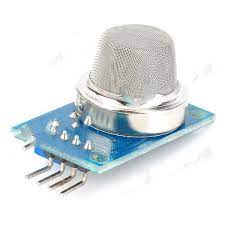
\includegraphics[]{images/FC22.png}\\
\caption{\emph{FC22}}
\end{center}
\emph{FC22}: Il sensore \emph{FC22} è responsabile della raccolta dati relativa a fumo e vapori infiammabili (ovviamente presenti nell’aria). Il risultato mostrato è espresso in ppm ovvero parti per milione: microgrammi (di una determinata sostanza) su metro cubo ($\frac{\mu g}{m^3}$).
\begin{center}
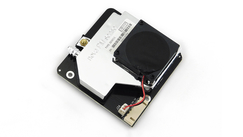
\includegraphics[]{images/sds011.jpg}\\
\caption{\emph{SDS011}}
\end{center}
\emph{SDS011}: Per ultimo abbiamo il rilevatore di polveri sottili, che ci restituisce il risultato sempre in microgrammi su metro cubo.\\
Il valore del PM2,5 indica la quantità di particelle con un diametro di 2,5 micron mentre PM10 ci indica la quantità di particelle con un diametro di 10 micron.
\section{Il sito}
La realizzazione del sito web, dove chiunque possa vedere i nostri dati, è principalmente dovuto all’enorme aiuto di un altro studente del Liceo che non ha preso parte all’intero progetto: Mattia Mascarello.\\
I dati sono elaborati in grafici a linee che spaziano nel giorno corrente, in quello precedente, nella settimana corrente e quella antecedente, con la possibilità di esportare dati d'archivio.\\
\subsection{Il software}
I dati vengono ricevuti con un codice di autorizzazione e vengono automaticamente archiviate, disponibili per l'elaborazione grafica e la ricerca ed esportazione in diversi formati.
\section{Video}

Il montaggio del video, nonché idea,  è stato realizzato grazie al prezioso aiuto di uno dei ragazzi che ha preso parte al progetto: Lorenza Dellapiana.
Il video è stato girato nei locali sia interni che esterni della scuola in cui alcuni studenti del programma hanno spiegato le varie vicissitudini e passaggi che li hanno portato fino alla fine di questa esperienza. Il video è particolarmente rivolto alle classi del biennio sempre per motivi didattici ma anche per invogliarli a prendere parte a progetti come questo.
\section{Posizione}
L' \emph{Aula del Cielo} è un progetto PCTO dell’anno scolastico 2020/2021, ideato da due docenti di scienze del liceo prof. Claudia Abrigo e prof. Loredana Ercolini, a cui hanno partecipato venti studenti delle classi terze e quarte.\\
Obiettivo del progetto è stato realizzare  nel giardino interno della scuola una zona dedicata alla misura di fenomeni atmosferici e astronomici, una vera “Aula del Cielo”. \\
L’aiuola del giardino è diventata una rosa dei venti, sulle pareti dell’edificio sono state costruite due meridiane, decorate con l’aiuto della professoressa Barale, e diversi orologi solari e camere stenopeiche sono ora a disposizione per osservazioni e misure.\\
Nell’\emph{Aula del cielo} sarà anche collocata la stazione meteo da noi realizzata per la raccolta di dati atmosferici ed ambientali.

\section{Open Source}
Tutto il codice del progetto è open source e pubblicato al seguente link\\
\url{https://github.com/MatMasIt/weatherStation}
\pagebreak
\renewcommand{\abstractname}{Riconosimenti}
\begin{center}
\begin{abstract}
Un sincero ringraziamento va a:\\
\textbf{Docenti}\\
 prof. Claudia Abrigo, Scienze\\
 prof. Loredana Ercolini, Scienze\\
 prof. Daniela Genta, Matematica e Fisica\\
 prof. Andrea Piccione, Matematica e Fisica\\
\textbf{Studenti}\\
Leonardo Agnoletto, 4G\\
Luca Savio Biello, 4G\\
Lorenzo Dellapiana, 4G\\
Arsildo Gjoka, 4G\\
Gaia Gnecchi, 5D\\
Mattia Mascarello, 5E\\
Elia Taliano, 4G
\end{abstract}
\end{center}
\end{document}
